\section{my\_help2hikiとは}
個々のユーザが独自のメモを作ることのできるgem,my\_helpを利用して作成した
メモをwikiへ自動変換することで,個人のメモを互いに見れるようにし,
研究室内で情報を共有する.

\section{コマンド}\begin{description}
\item[TARGET --push]  作成したメモ(TARGET)をサーバに送る

\item[my\_help --hiki]  作成したメモをhiki形式に変換し,wikiで表示できるようにする.

\end{description}
\subsection{コマンドの振る舞い}
\subsubsection{TARGET --push}\begin{quote}\begin{verbatim}
date_dir = File.join(ENV['HOME'],'.my_help')
FileUtils.cd(data_dir)
system "rm -rf ~/.my_help/*.yml~"
system "scp -r ~/.my_help saki@nishitani0:~"
system "ssh saki@nishitani0 ls ~/.my_help"
\end{verbatim}\end{quote}
\begin{itemize}
\item 1,2行目
\end{itemize}
my\_helpでは,作成したメモが.my\_helpのディレクトリに自動的に追加されるので,
ディレクトリを.my\_helpに移動する.

\begin{itemize}
\item 3行目
\end{itemize}
.my\_helpにメモが追加されるとき,yaml形式のファイルで保存される.
メモを更新すると,一つ前に保存したファイルは*.yml~というファイル名
でバックアップとして残される.
\textbf{rm -rf}で不必要なファイルは削除し,サーバにコピーするときのデータ量を減らしている.

\begin{itemize}
\item 4行目
\end{itemize}
\textbf{scp -r ~/[directory名] [server名]}
serverにssh接続を行い,directoryをserverにコピーする.
-rはディレクトリ全体をコピーすることを示している.
西谷研究室で利用しているnishitani0というサーバにコピーしている.

\begin{itemize}
\item 失敗例
\end{itemize}
ターミナルでこのコマンドを使わずにコピーする場合
\begin{quote}\begin{verbatim}
/Users/saki/my_help% ssh nishitani0
Last login: Mon Jan  2 22:16:29 2017 from 59x87x69x163.ap59.ftth.ucom.ne.jp
[nishitani0:~] saki% cp -r ~/.my_help saki@nishitani0
[nishitani0:~] saki% exit
logout
Connection to nishitani0 closed.
\end{verbatim}\end{quote}
上記にようにすると,sshで接続し.my\_helpをdirectoryをcpを使ってコピー,
ssh接続を切るという作業を1行ずつ行うことができる.
同じようにコマンドの中身を下記のようにした.
\begin{quote}\begin{verbatim}
system "ssh nishitani0"
system "cp -r ~/.my_help saki@nishitani0"
system "exit"
\end{verbatim}\end{quote}
実行結果
\begin{quote}\begin{verbatim}
/Users/saki/my_help% bundle exec exe/my_todo --push
Last login: Sat Jan 28 03:49:46 2017 from 59x87x69x163.ap59.ftth.ucom.ne.jp
[nishitani0:~] saki% 
\end{verbatim}\end{quote}
このように1行目のみ実行したところで終了してしまった.
ssh接続を行うと,その後の命令は全てserver側で実行されることになるため,
1行ずつ行うと途中でターミナルでは実行ができなくなってしまいうまくいかない.

\begin{itemize}
\item 失敗例2
\end{itemize}
\textbf{ssh [server名] [command]}とするとserverにsshで接続してcommandを実行し
ログアウトすることができるため,以下のように書き換えた.
\begin{quote}\begin{verbatim}
system "ssh nishitani0 cp ~/.my_help saki@nishitani0"
\end{verbatim}\end{quote}
実行結果
\begin{quote}\begin{verbatim}
/Users/saki/my_help% bundle exec exe/my_todo --push
cp: /Users/saki/.my_help is a directory (not copied).
\end{verbatim}\end{quote}
sshでファイルやディレクトリをコピーするコマンドはcpではなくscpなので,
実行することができなかった.

\begin{itemize}
\item 5行目
\end{itemize}
nishitani0にssh接続し.my\_helpの中身を書き出して,
コピーができているかコマンドを実行した時に確認が行えるようにしている.

\subsubsection{my\_help --hiki}\begin{quote}\begin{verbatim}
system "emacs_help --to_hiki > ~/Sites/hiki-1.0/data/text/emacs_help_saki"
system "my_todo --to_hiki > ~/Sites/hiki-1.0/data/text/my_todo_saki"
system "ssh_help --to_hiki > ~/Sites/hiki-1.0/data/text/ssh_help_saki"
system "open -a safari 'http://localhost/~saki/hiki-1.0/?FrontPage'"
\end{verbatim}\end{quote}
\begin{itemize}
\item 1~3行目
\end{itemize}
my\_helpには,\textbf{TARGET --to\_hiki}というコマンドがあり,これによって
yaml形式で保存されているメモをhiki形式で書き出すことができる.
この --hiki のコマンドを使ってhiki形式にしたものを,wikiで表示することのできる
フォルダである\textbf{~/Sites/hiki-1.0/data/text/}に入れることで,wikiでの表示を可能にしている.
emacs\_help,my\_todo,ssh\_helpは全て私のmy\_helpに入っているメモ.

\begin{itemize}
\item 4行目
\end{itemize}
wikiのページ\textbf{FrontPage}を表示するコマンド.
これによりメモが更新されているのを即時確認することができる.
FrontPageは以下のようになっている.
\begin{quote}\begin{verbatim}
!saki's help
*[[ssh_help_saki]]
*[[my_todo_saki]]
*[[emacs_help_saki]]
\end{verbatim}\end{quote}
先頭に\textbf{!}をつけることで1行目のsaki's helpを見出しにし,
2~4行目は\textbf{*}によって箇条書き,角括弧でリンクになっている.

\subsection{利便性}
メモを更新してから,上記の2つのコマンドを共に行うと,
自分のmy\_helpにあるメモ,サーバのバックアップ,
研究室内のメンバーが見ることのできるwikiの全てが同じ内容になる.
研究室内全員が同じ情報を得ることで,情報を共有するという目標が達成できる.
また,メモをすべてmy\_helpで作成しておけば,忘れてしまったときに
my\_helpのみを確認すればよく,管理が楽になる.
gemの開発中や課題の途中にもすぐメモを残すことができるので,
それぞれのユーザが得た暗黙知もすぐに形式知化することが可能になることが
期待される.

\begin{figure}[htbp]\begin{center}
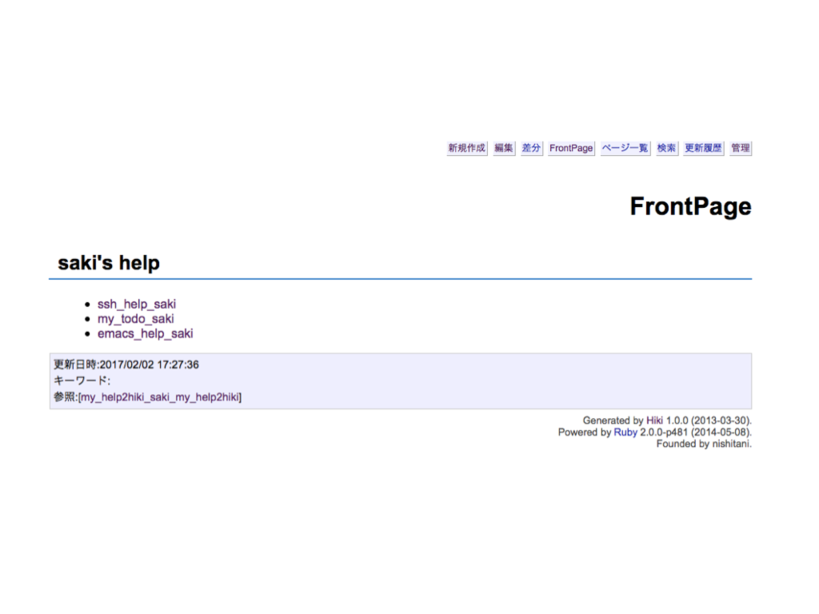
\includegraphics[width=6cm,bb=0 0 442 500]{../figs/./my_help2hiki_saki.002.png}
\caption{}
\label{default}\end{center}\end{figure}
\begin{table}[htbp]\begin{center}
\caption{}
\begin{tabular}{ll}
\hline
\fig{my\_help2hiki\_saki.002} コマンドを実行したときに開くFrontPage  \\ \hline
\hline
\end{tabular}
\label{default}
\end{center}\end{table}
%for inserting separate lines, use \hline, \cline{2-3} etc.

